
In this section, we are going to learn about Clang's AST in-memory representation and its essential API usage. The first part of this section will provide you with a high-level overview of Clang AST's hierarchy; the second part will focus on a more specific topic regarding type representation in Clang AST; and the final part will show you the basic usage of AST matcher, which is extremely useful when you're writing an AST plugin.

\subsubsubsection{7.2.1\hspace{0.2cm}In-memory structure of Clang AST}

The in-memory representation of AST in Clang is organized in a hierarchy structure that resembles the syntax structure of C-family language programs. Starting from the top-most level, there are two classes worth mentioning:

\begin{itemize}
\item TranslationUnitDecl: This class represents an input source file, also called a translation unit (most of the time). It contains all the top-level declarations – global variables, classes, and functions, to name a few – as its children, where each of those top-level declarations has its own subtree that recursively defines the rest of the AST.

\item ASTContext: As its name suggests, this class keeps track of all the AST nodes and other metadata from the input source files. If there are multiple input source files, each of them gets its own TranslationUnitDecl, but they all share the same ASTContext.
\end{itemize}

In addition to the structure, the body of the AST – the AST nodes – can be further classified into three primary categories: declaration, statement, and expression. The nodes in these categories are represented by subclasses derived from the Decl, Expr, and Stmt classes, respectively. In the following sections, we are going to introduce each of these in-memory AST representations.

\hspace*{\fill} \\ %插入空行
\noindent
\textbf{Declarations}

Language constructs such as variable declarations (global and local), functions, and struct/class declarations are represented by subclasses of Decl. Though we are not going to go into each of these subclasses here, the following diagram shows common declaration constructions in C/C++ and their corresponding AST classes:

\hspace*{\fill} \\ %插入空行
\begin{center}
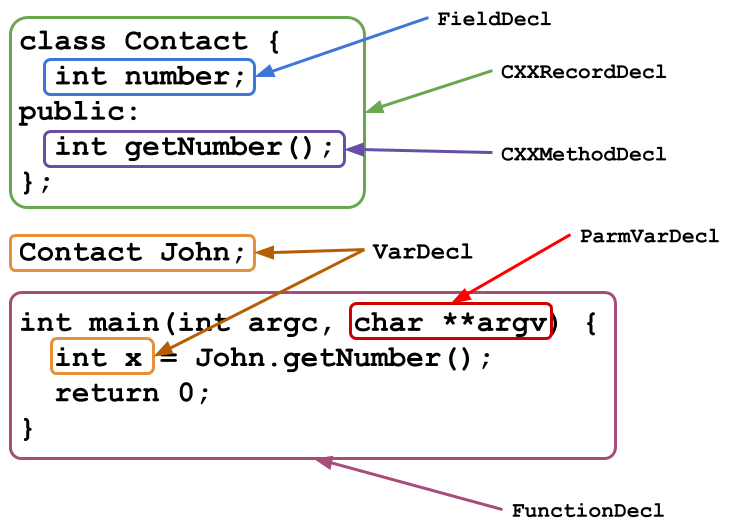
\includegraphics[width=0.9\textwidth]{content/2/chapter7/images/1.png}\\
Figure 7.1 – Common declarations in C/C++ and their AST classes
\end{center}

Between more concrete subclasses, such as FunctionDecl and Decl, there are several important abstract classes that represent certain language concepts:

\begin{itemize}
\item NamedDecl: For every declaration that has a name.
\item ValueDecl: For declarations whose declared instances can be a value, and thus are associated with type information.
\item WDeclaratorDecl: For every declaration that uses declarator (basically a statement in the form of <type and qualifier> <identifier name>). They provide extra information about parts other than the identifier. For example, they provide access to an in-memory object with namespace resolution, which acts as a qualifier in the declarator.
\end{itemize}

To learn more about AST classes for other kinds of declarations, you can always navigate through the subclasses of Decl on LLVM's official API reference website.

\hspace*{\fill} \\ %插入空行
\noindent
\textbf{Statements}

Most directives in a program that represent the concept of actions can be classified as statements and are represented by subclasses of Stmt, including expressions, which we are going to cover shortly. In addition to imperative statements such as function calls or return sites, Stmt also covers structural concepts such as for loops and if statements. Here is a diagram showing a common language construct represented by Stmt (except expression) in C/C++ and its corresponding AST classes:


\hspace*{\fill} \\ %插入空行
\begin{center}
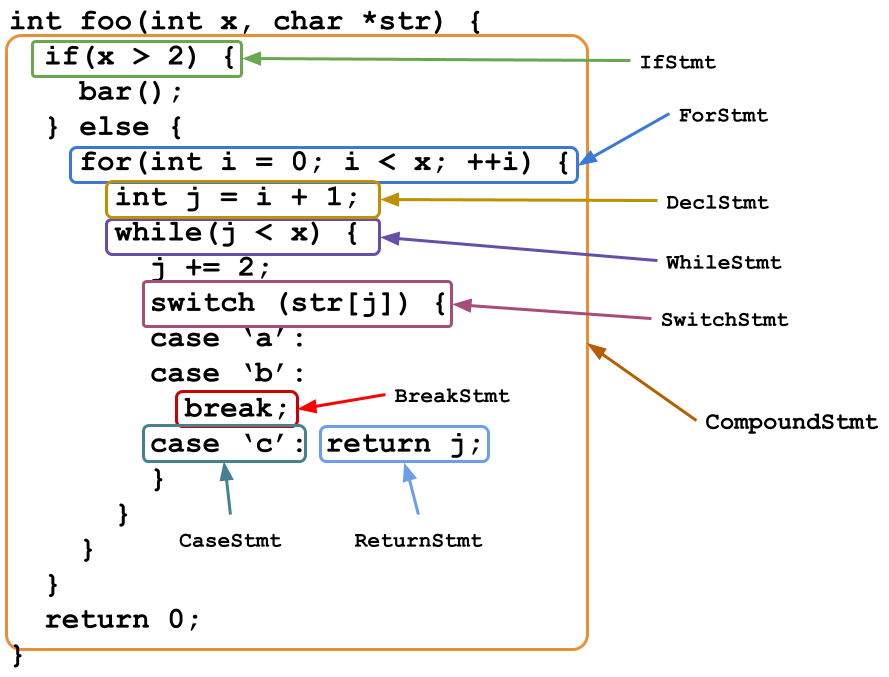
\includegraphics[width=0.9\textwidth]{content/2/chapter7/images/2.png}\\
Figure 7.2 – Common statements (excluding expressions) in C/C++ and their AST classes
\end{center}

There are two things worth mentioning about the previous diagram:

\begin{itemize}
\item CompoundStmt, which is a container for multiple statements, represents not only the function body but basically any code block enclosed by curly braces ('\{', '\}'). Therefore, though not shown in the preceding diagram due to a lack of space, IfStmt, ForStmt, WhileStmt, and SwitchStmt all have a CompoundStmt child node representing their bodies.

\item Declarations in a CompoundStmt will be wrapped by a DeclStmt node, in which the real Decl instance is its child node. This creates a simpler AST design.
\end{itemize}

Statements are one of the most prevailing directives in a typical C/C++ program. It is worth noting, however, that many statements are organized in a hierarchy (for example, ForStmt and its loop body), so it might take you extra steps to go down this hierarchy before you find the desired Stmt node.

\hspace*{\fill} \\ %插入空行
\noindent
\textbf{Expressions}

Expressions in Clang AST are a special kind of statement. Different from other statements, expressions always generate values. For example, a simple arithmetic expression, 3 + 4, is expected to generate an integer value. All expressions in Clang AST are represented by subclasses of Expr. Here is a diagram showing a common language construct represented by Expr in C/C++ and its corresponding AST classes:

\hspace*{\fill} \\ %插入空行
\begin{center}
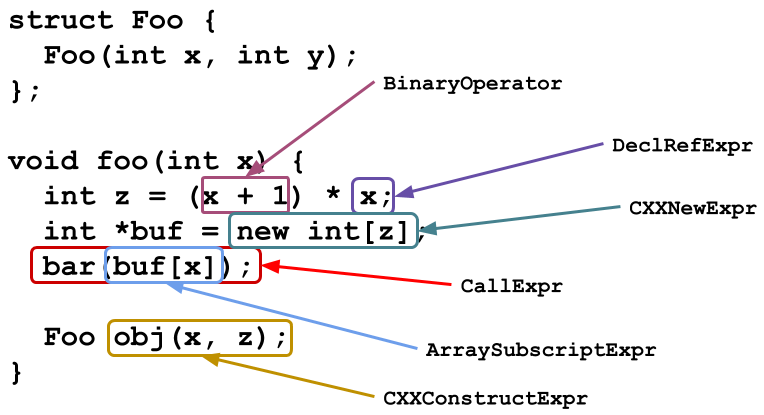
\includegraphics[width=0.9\textwidth]{content/2/chapter7/images/3.png}\\
Figure 7.3 – Common expressions in C/C++ and their AST classes
\end{center}

One important Expr class is DeclRefExpr. It represents the concept of symbol reference. You can use one of its APIs, DeclRefExpr::getDecl(), to retrieve the referenced symbol's Decl object. Handy symbol information like this only appears after AST has been generated, so this is one of the reasons people always recommend implementing static analysis logic on AST rather on more primitive forms (inside the parser, for example).

Another interesting Expr class – not highlighted in the preceding diagram due to a lack of space – is ParenExpr, which represents the parentheses that wrap around an expression. For example, in the preceding diagram, (x + 1) is a ParenExpr with a BinaryOperator representing x + 1 as its child.

\subsubsubsection{7.2.2\hspace{0.2cm}Types in Clang AST}

The type system is one of the most crucial components in modern compilers, especially for statically typed languages such as C/C++. Type checking ensures that the input source code is well-formed (to some extent) and catches as many errors as possible at compile time. While we don't need to do type checking by ourselves in Clang, it is done by the Sema subsystem, which we introduced in Chapter 5, Exploring Clang's Architecture. You will probably need to leverage this information when you're processing the AST. Let's learn how types are modeled in Clang AST.

\hspace*{\fill} \\ %插入空行
\noindent
\textbf{Core classes}

The core of Clang AST's type system is the clang::Type class. Each type in the input code – including primitive types such as int and user-defined types such as struct/class – is represented by a singleton type (more specifically, a subclass of Type) object.

\begin{tcolorbox}[colback=blue!5!white,colframe=blue!75!black, fonttitle=\bfseries,title=Terminology]
\hspace*{0.7cm}In the rest of this chapter, we will call types in the input source code source code types.
\end{tcolorbox}

A singleton is a design pattern that forces a resource or an abstract concept to be represented by only one in-memory object. In our case, source code types are the resources, so you will find only one Type object for each of those types. One of the biggest advantages of this design is that you have an easier way to compare two Type objects. Let's say you have two Type pointers. By doing a simple pointer comparison (which is extremely fast) on them, you can tell if they're representing the same source code type.

\begin{tcolorbox}[colback=blue!5!white,colframe=blue!75!black, fonttitle=\bfseries,title=Counter Example of a Singleton Design]
\hspace*{0.7cm}If Type in Clang AST is not using a singleton design, to compare if two Type pointers are representing the same source code types, you need to inspect the content of the objects they are pointing to, which is not efficient.
\end{tcolorbox}

As we mentioned earlier, each source code type is actually represented by a subclass of Type. Here are some common Type subclasses:

\begin{itemize}
\item BuiltinType: For primitive types such as int, char, and float.

\item PointerType: For all the pointer types. It has a function called PointerType::getPointee() for retrieving the source code type being pointed to by it.

\item ArrayType: For all the array types. Note that it has other subclasses for more specific arrays that have either a constant or variable length.

\item RecordType: For struct/class/union types. It has a function called RecordType::getDecl() for retrieving the underlying RecordDecl.

\item FunctionType: For representing a function's signature; that is, a function's argument types and return type (and other properties, such as its calling convention).

\end{itemize}

Let us now move on to the qualified types.

\hspace*{\fill} \\ %插入空行
\noindent
\textbf{Qualified types}

One of the most confusing things for people new to Clang's code base is that many places use the QualType class rather than subclasses of Type to represent source code types. QualType stands for qualified type. It acts as a wrapper around Type to represent concepts such as const <type>, volatile <type>, and restrict <type>*.

To create a QualType from a Type pointer, you can use the following code:

\begin{lstlisting}[style=styleCXX]
// If `T` is representing 'int'…
QualType toConstVolatileTy(Type *T) {
	return QualType(T, Qualifier::Const | Qualifier::Volatile);
} // Then the returned QualType represents `volatile const int`
\end{lstlisting}

In this section, we learned about the type system in Clang AST. Let's now move on to ASTMatcher, a syntax to match patterns.

\subsubsubsection{7.2.3\hspace{0.2cm}ASTMatcher}

When we are dealing with a program's AST – for example, we're checking if there is any suboptimal syntax – searching for specific AST nodes pattern is usually the first step, and one of the most common things people do. Using the knowledge we learned in the previous section, we know that this kind of pattern matching can be done by iterating through AST nodes via their in-memory classes APIs. For example, given a FunctionDecl – the AST class of a function – you can use the following code to find out if there is a while loop in its body and if the exit condition of that loop is always a literal Boolean value; that is, true:

\begin{lstlisting}[style=styleCXX]
// `FD` has the type of `const FunctionDecl&`
const auto* Body = dyn_cast<CompoundStmt>(FD.getBody());
for(const auto* S : Body->body()) {
	if(const auto* L = dyn_cast<WhileStmt>(S)) {
		if(const auto* Cond = dyn_cast<CXXBoolLiteralExpr>
		(L->getCond()))
		if(Cond->getValue()) {
			// The exit condition is `true`!!
		}
	}
}
\end{lstlisting}

As you can see, it created more than three (indention) layers of if statements to complete such a simple check. Not to mention in real-world cases, we need to insert even more sanity checks among these lines! While Clang's AST design is not hard to understand, we need a more concise syntax to complete pattern matching jobs. Fortunately, Clang has already provided one – the ASTMatcher.

ASTMatcher is the utility that helps you write AST pattern matching logic via a clean, concise, and efficient Domain-Specific Language (DSL). Using ASTMatcher, doing the same matching shown in the previous snippet only takes few lines of code:

\begin{lstlisting}[style=styleCXX]
functionDecl(compountStmt(hasAnySubstatement(
  whileStmt(
    hasCondition(cxxBoolLiteral(equals(true)))))));
\end{lstlisting}

Most of the directives in the preceding snippet are pretty straightforward: function calls such as compoundStmt(…) and whileStmt(…) check if the current node matches a specific node type. Here, the arguments in these function calls either represent pattern matchers on their subtree or check additional properties of the current node. There are also other directives for expressing qualifying concepts (for example, for all substatements in this loop body, a return value exists), such as hasAnySubstatement(…), and directives for expressing data type and constant values such as the combination of cxxBoolLiteral(equals(true)).

In short, using ASTMatcher can make your pattern matching logic more expressive. In this section, we showed you the basic usage of this elegant DSL.

\hspace*{\fill} \\ %插入空行
\noindent
\textbf{Traversing AST}

Before we dive into the core syntax, let's learn how ASTMatcher traverses AST and how it passes the result back to users after the matching process is completed. 

MatchFinder is a commonly used driver for the pattern matching process. Its basic usage is pretty simple:

\begin{lstlisting}[style=styleCXX]
using namespace ast_matchers;
…
MatchFinder Finder;
// Add AST matching patterns to `MatchFinder`
Finder.addMatch(traverse(TK_AsIs, pattern1), Callback1);
Finder.addMatch(traverse(TK_AsIs, pattern2), Callback2);
…
// Match a given AST. `Tree` has the type of `ASTContext&`
// If there is a match in either of the above patterns,
// functions in Callback1 or Callback2 will be invoked
// accordingly
Finder.matchAST(Tree);

// …Or match a specific AST node. `FD` has the type of
// `FunctionDecl&`
Finder.match(FD, Tree);
\end{lstlisting}

pattern1 and pattern2 are pattern objects that are constructed by DSL, as shown previously. What's more interesting is the traverse function and the TK\_AsIs argument. The traverse function is a part of the pattern matching DSL, but instead of expressing patterns, it describes the action of traversing AST nodes. On top of that, the TK\_AsIs argument represents the traversing mode.

When we showed you the command-line flag for dumping AST in textual format (-Xclang -ast-dump) earlier in this chapter, you may have found that many hidden AST nodes were inserted into the tree to assist with the program's semantics rather than representing the real code that was written by the programmers. For example, ImplicitCastExpr is inserted in lots of places to ensure the program's type correctness. Dealing with these nodes might be a painful experience when you're composing pattern matching logic. Thus, the traverse function provides an alternative, simplified, way to traverse the tree. Let's say we have the following input source code:

\begin{lstlisting}[style=styleCXX]
struct B {
	B(int);
};
B foo() { return 87; }
\end{lstlisting}

When you pass TK\_AsIs as the first argument to traverse, it observes the tree, similar to how -ast-dump does:

\begin{tcblisting}{commandshell={}}
FunctionDecl
`-CompoundStmt
  `-ReturnStmt
    `-ExprWithCleanups
      `-CXXConstructExpr
        `-MaterializeTemporaryExpr
          `-ImplicitCastExpr
            `-ImplicitCastExpr
              `-CXXConstructExpr
                `-IntegerLiteral 'int' 87
\end{tcblisting}

However, by using TK\_IgnoreUnlessSpelledInSource as the first argument, the tree that's observed is equal to the following one:

\begin{tcblisting}{commandshell={}}
FunctionDecl
`-CompoundStmt
  `-ReturnStmt
    `-IntegerLiteral 'int' 87
\end{tcblisting}

As its name suggests, TK\_IgnoreUnlessSpelledInSource only visit nodes that are really shown in the source code. This greatly simplifies the process of writing a matching pattern since we don't need to worry about the nitty-gritty details of AST anymore.

On the other hand, Callback1 and Callback2 in the first snippet are MatchFinder::MatchCallback objects that describe the actions to perform when there is a match. Here is the skeleton of a MatchCallback implementation:

\begin{lstlisting}[style=styleCXX]
struct MyMatchCallback : public MatchFinder::MatchCallback {
	void run(const MatchFinder::MatchResult &Result) override {
		// Reach here if there is a match on the corresponding
		// pattern
		// Handling "bound" result from `Result`, if there is any
	}
};
\end{lstlisting}

In the next section, we will show you how to bind a specific part of the pattern with a tag and retrieve it in MatchCallback.

Last but not least, though we used MatchFinder::match and MatchFinder::matchAST in the first snippet to kick off the matching process, there are other ways to do this. For example, you can use MatchFinder::newASTConsumer to create an ASTConsumer instance that will run the described pattern matching activity. Alternatively, you can use ast\_matchers::match(…) (not a member function under MatchFinder but a standalone function) to perform matching on a provided pattern and ASTContext in a single run, before returning the matched node.

\hspace*{\fill} \\ %插入空行
\noindent
\textbf{ASTMatcher DSL}

ASTMatcher provides an easy-to-use and concise C++ DSL to help with matching AST. As we saw earlier, the structure of the desired pattern is expressed by nested function calls, where each of these functions represents the type of AST node to match.

Using this DSL to express simple patterns cannot be easier. However, when you're trying to compose patterns with multiple conditions/predicates, things get a little bit more complicated. For example, although we know a for loop (for example, for(I = 0; I < 10; ++I){…}) can be matched by the forStmt(…) directive, how do we add a condition to its initialize statement (I = 0 ) and exit the condition (I < 10) or its loop body? Not only does the official API reference site (the doxygen website we usually use) lacks clear documentation on this part, most of these DSL functions are also pretty flexible in how they accept a wide range of arguments as their subpatterns. For example, following the question on matching a for loop, you can use the following code to check only the loop's body:

\begin{lstlisting}[style=styleCXX]
forStmt(hasBody(…));
\end{lstlisting}

Alternatively, you can check its loop body and its exit condition, like so:

\begin{lstlisting}[style=styleCXX]
forStmt(hasBody(…),
  hasCondition(…));
\end{lstlisting}

A generalized version of this question would be, given an arbitrary DSL directive, how do we know the available directives that can be combined with it?

To answer this question, we will leverage a documentation website LLVM specifically created for ASTMatcher: \url{https://clang.llvm.org/docs/LibASTMatchersReference.html}. This website consists of a huge three-column table showing the returned type and argument types for each of the DSL directives:

\hspace*{\fill} \\ %插入空行
\begin{center}
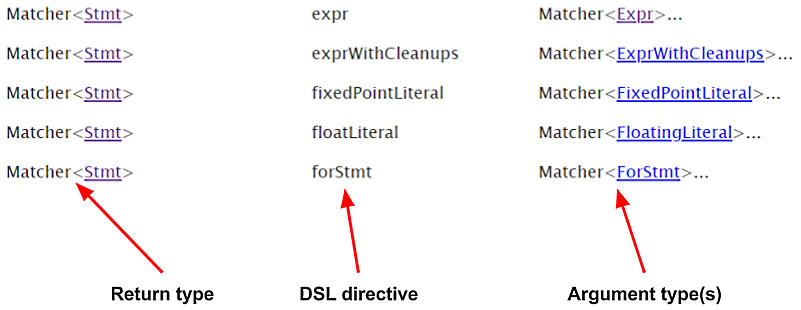
\includegraphics[width=0.9\textwidth]{content/2/chapter7/images/4.png}\\
Figure 7.4 – Part of the ASTMatcher DSL reference
\end{center}

Though this table is just a simplified version of normal API references, it already shows you how to search for candidate directives. For example, now that you know forStmt(…) takes zero or multiple Matcher<ForStmt>, we can search this table for directives that return either Matcher<ForStmt> or Matcher<(parent class of ForStmt)>, such as Matcher<Stmt>. In this case, we can quickly spot hasCondition, hasBody, hasIncrement, or hasLoopInit as candidates (of course, many other directives that return Matcher<Stmt> can also be used).

When you're performing pattern matching, there are many cases where you not only want to know if a pattern matches or not but also get the matched AST nodes. In the context of ASTMatcher, its DSL directives only check the type of the AST nodes. If you want to retrieve (part of the) concrete AST nodes that are being matched, you can use the bind(…) API. Here is an example:

\begin{lstlisting}[style=styleCXX]
forStmt(
  hasCondition(
    expr().bind("exit_condition")));
\end{lstlisting}

Here, we used expr() as a wildcard pattern to match any Expr node. This directive also calls bind(…) to associate the matched Expr AST node with the name exit\_condition.

Then, in MatchCallback, which we introduced earlier, we can retrieve the bound node by using the following code:

\begin{lstlisting}[style=styleCXX]
…
void run(const MatchFinder::MatchResult &Result) override {
	cons auto& Nodes = Result.Nodes;
	const Expr* CondExpr = Nodes.getNodeAs<Expr>
	("exit_condition");
	// Use `CondExpr`…
}
\end{lstlisting}

The getNodeAs<…>(…) function tries to fetch the bound AST node under the given name and cast it to the type suggested by the template argument. 

Note that you're allowed to bind different AST nodes under the same name, in which case only the last bounded one will be shown in MatchCallback::run.

\hspace*{\fill} \\ %插入空行
\noindent
\textbf{Putting everything together}

Now that you've learned about both the pattern matching DSL syntax and how to traverse AST using ASTMatcher, let's put these two things together.

Let's say we want to know the number of iterations – also known as the trip count – that a simple for loop (the loop index starts from zero and is incremented by one at each iteration and bounded by a literal integer) has in a function:

\begin{enumerate}
\item First, we must write the following code for matching and traversing:

\begin{lstlisting}[style=styleCXX]
auto PatExitCondition = binaryOperator(
                           hasOperatorName("<"),
                           hasRHS(integerLiteral()
                           .bind("trip_count")));
auto Pattern = functionDecl(
                  compountStmt(hasAnySubstatement(
               forStmt(hasCondition(PatExitCondition)))));
               
MatchFinder Finder;
auto* Callback = new MyMatchCallback();
Finder.addMatcher(traverse(TK_IgnoreUnlessSpelledInSource,
                           Pattern), Callback);
\end{lstlisting}

The preceding snippet also shows how modular DSL patterns are. You can create individual pattern fragments and compose them depending on your needs, as long as they're compatible.

Finally, here is what MyMatchCallback::run looks like:

\begin{lstlisting}[style=styleCXX]
void run(const MatchFinder::MatchResult &Result) override
{
	const auto& Nodes = Result.Nodes;
	const auto* TripCount =
	Nodes.getNodeAs<IntegerLiteral>("trip_count");
	if (TripCount)
	TripCount->dump(); // print to llvm::errs()
}
\end{lstlisting}

\item After this, you can use Finder to match the desired pattern (either by calling MatchFinder::match or MatchFinder::matchAST, or by creating an ASTConsumer using MatchFinder::newASTConsumer) on an AST. The matched trip count will be printed to stderr. For instance, if the input source code is for(int i = 0; i < 10; ++i) {…}, the output will simply be 10.
\end{enumerate}

In this section, we learned how Clang structures its AST, how Clang AST is represented in memory, and how to use ASTMatcher to help developers with AST pattern matching. With this knowledge, in the next section, we will show you how to create an AST plugin, which is one of the easiest ways to inject custom logic into Clang's compilation pipeline.





















